%%
%% This is file `sample-sigconf.tex',
%% generated with the docstrip utility.
%%
%% The original source files were:
%%
%% samples.dtx  (with options: `sigconf')
%% 
%% IMPORTANT NOTICE:
%% 
%% For the copyright see the source file.
%% 
%% Any modified versions of this file must be renamed
%% with new filenames distinct from sample-sigconf.tex.
%% 
%% For distribution of the original source see the terms
%% for copying and modification in the file samples.dtx.
%% 
%% This generated file may be distributed as long as the
%% original source files, as listed above, are part of the
%% same distribution. (The sources need not necessarily be
%% in the same archive or directory.)
%%
%% The first command in your LaTeX source must be the \documentclass command.
\documentclass[sigconf]{acmart}

%%
%% \BibTeX command to typeset BibTeX logo in the docs
\AtBeginDocument{%
  \providecommand\BibTeX{{%
    \normalfont B\kern-0.5em{\scshape i\kern-0.25em b}\kern-0.8em\TeX}}}

%%
%% Submission ID.
%% Use this when submitting an article to a sponsored event. You'll
%% receive a unique submission ID from the organizers
%% of the event, and this ID should be used as the parameter to this command.
%%\acmSubmissionID{123-A56-BU3}

%%
%% The majority of ACM publications use numbered citations and
%% references.  The command \citestyle{authoryear} switches to the
%% "author year" style.
%%
%% If you are preparing content for an event
%% sponsored by ACM SIGGRAPH, you must use the "author year" style of
%% citations and references.
%% Uncommenting
%% the next command will enable that style.
%%\citestyle{acmauthoryear}

%%
%% end of the preamble, start of the body of the document source.
\begin{document}

%%
%% The "title" command has an optional parameter,
%% allowing the author to define a "short title" to be used in page headers.
\title{Exploring Generic and Semantic Profiling in Python for Data Mining}

%%
%% The "author" command and its associated commands are used to define
%% the authors and their affiliations.
%% Of note is the shared affiliation of the first two authors, and the
%% "authornote" and "authornotemark" commands
%% used to denote shared contribution to the research.
\author{Jack Li}
\affiliation{%
    \institution{New York University}
    \city{New York}
    \country{United States}
}
\email{ql1045@nyu.edu}

\author{TODO}
\affiliation{%
    \institution{New York University}
    \city{New York}
    \country{United States}
}
\email{TODO@nyu.edu}

\author{TODO}
\affiliation{%
    \institution{New York University}
    \city{New York}
    \country{United States}
}
\email{TODO@nyu.edu}


%%
%% By default, the full list of authors will be used in the page
%% headers. Often, this list is too long, and will overlap
%% other information printed in the page headers. This command allows
%% the author to define a more concise list
%% of authors' names for this purpose.

%%
%% The abstract is a short summary of the work to be presented in the
%% article.
\begin{abstract}
    With more complexity of datasets and greater emphasis on data quality, understanding the structure of the dataset has become one of the essential requirements before mining data. We applied data profiling tools to identify potential quality issues, examine the available data from testing datasets, and collect statistical information about them. For example, the recommendation engine has played a critical role in the online retail and entertainment industry and affected our daily life in different ways. The system generally deals with big data technology, which is composed of data collection, cleaning, profiling, and filtering. Hence, Data profiling is crucial for IT professionals and data researchers to analyze big data. 
    
    The report represents the data processing activities, including genetic profiling tasks and semantic types classification of each column. For task1, we examined and ran all 1900 files to output the generic profiling JSON files. For task2, we detected the different types and assigned one or more semantic type labels to each column. The purpose is to characterize and classify the data and generate informative summaries derived from whole subsets.
\end{abstract}

%%
%% Keywords. The author(s) should pick words that accurately describe
%% the work being presented. Separate the keywords with commas.
\keywords{datasets, profiling, senmatic, text tagging, data mining}

%%
%% This command processes the author and affiliation and title
%% information and builds the first part of the formatted document.
\maketitle

\section{Introduction}
In the real world, large parts of the data are interconnected and rational. With discovering errors within the datasets and verifying the data quality, IT researchers would be able to clarify if the datasets are reliable, consistent, accuracy, or Null. 
Meanwhile, with the high-speed network and inexpensive cost of storage, the enormous amount of data has been generated and stored every day. An efficient process for data profiling would not only save time and resources but improve the productivity of the project. 

In this project, we would first read the relevant reports and discuss the meanings of data profiling. Secondly, we worked on the first task is to figure out data types, statistical features of each column from giving datasets. Thirdly, we tried to classify the semantic model based on their characteristics of each column from the assigned datasets.

Data profiling through a series of processes has currently become one of the best methods when analyzing huge amounts of data, and also strengthen our data quality. Nowadays, the lack of high data quality will lead to weakening or discontinued business intelligence, and even lost the trust of Information consumers.

\section{Task 1}
In the first task, we profile a large amount of NYC open data as instructed. The framework we use is a powerful big data processing engine called Spark. To further ease our programming, we use the more recent dataframe API in replacement of the traditional RDD one. Dataframes enable named columns and simpler aggregations. It also employs catalyst optimizer to get a better execution plan than RDD. From the user's point of view, the interface is much like the widely used SQL which lowers the learning overhead. We load the dataset as a dataframe, let the framework decide a type for each column, and then dive into columns without a certain inference.
\\\\
We run our program on the NYU dumbo cluster. The first 200 instances finished in 2 hours, but the cluster soon got crowded as it is shared. During peak time the processing speed is about 10 instances per hour.
\\\\
We iterate through all filenames and titles as in the index file \verb|datasets.tsv| provided by the datasets. Integers and floats are trivial to detect, and spark can detect them quite precisely. The rest columns will be assigned type \verb|TEXT|. This is where more fine-tuned logic happens.
\\\\
For the \verb|data_types| attribute, we implement a \verb|profile_datatype| function to identify specific data types for columns containing the different type values. To identify the column with the value of type DATE, we turn to the existing library \verb|dateparser| for help. This Python library provides a highly adaptable parser module that handles loosely formatted date-time pretty well. As for numeric values, we will try to cast them into integer or float. If it succeeds, we will classify that value as integer or float.
\\\\
We also encountered some challenges and issues in the implementation of general profiling. As referred above, columns with \verb|date/time| are generally heterogeneous and are mixed up with values of multiple types. For task 1, one of the most common problems we face is handling dates and times. With the help of the aforementioned parser library, we can extract a well-formed representation from the \verb|date/time| text. With the help of \verb|to_iso_string| function, we can further convert it into a standard ISO form without ambiguity. This ISO string serves as a common language between the parser and spark. We can then perform more detailed analyses on the data.
\\\\
The next issue we face is about data quality. Dots are not legitimate symbols in spark columns, but some raw data contains dots as column names. The workaround we propose is to wrap such column names with extra quoting to prevent the spark from messing up different entities. 
\\\\
Next, some datasets have non-ASCII column names. Certain string manipulation such as regular expression, character count or JSON dumping may crash if without proper encoding. We have set up extra environments to convert everything into the correct representation.
\\\\
Our first implementation has acceptable speed, but soon it gets slower as the usage of the cluster multiplies. In the optimization process, we found that every python spark function call introduces some overhead since it involves python-java context switches. To speed up our code, we reduced such overheads by grouping as many queries together as possible. 
\\\\
The results of our profiling task is shown in table \ref{tk1tb}. Most common is \verb|TEXT| type as it is the fallback if no other more specific types can be assigned. The second on is \verb|INTEGER (LONG)| which is neither surprising because integer is an intuitive choice for enumeration or indexing.
\\\\
\begin{figure}[h]
    \centering
    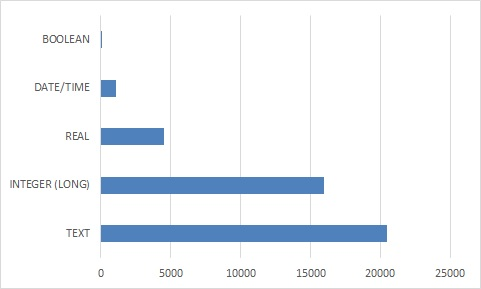
\includegraphics[width=0.45\textwidth]{num_of_each_datatype.jpg}
    \caption{Number of Columns for Each Data Type}
    \label{fig:mesh1}
\end{figure}
\begin{table}[h]
    \centering
    \begin{tabular}{ |c|c| }
        \hline
        type & columns containing this type \\
        \hline
        TEXT & 20478 \\
        INTEGER (LONG) & 15919 \\
        DATE/TIME & 1053 \\
        REAL & 4503 \\
        BOOLEAN & 70 \\
        \hline
    \end{tabular}
    \caption{Task 1 statistics}
    \label{tk1tb}
\end{table}
The most common types that co-occur in columns is \verb|INTEGER (LONG)|, \verb|TEXT|. This is possibly due to their large priori.
\\\\
\begin{table}[h]
    \centering
    \begin{tabular}{ |c|c| }
        \hline
        combination & count \\
        \hline
        INTEGER (LONG),TEXT & 5661 \\
        DATE/TIME,TEXT & 933 \\
        INTEGER (LONG),REAL,TEXT & 354 \\
        DATE/TIME,INTEGER (LONG),REAL,TEXT & 74 \\
        REAL,TEXT & 64 \\
        DATE/TIME,REAL,TEXT & 17 \\
        \hline
    \end{tabular}
    \caption{Task 1 co-occur}
    \label{tk1cooc}
\end{table}
We find that common representation for missing values includes values as in table \ref{msvltb}. There are 7103 heterogeneous columns in total in the datasets.
\\\\
\begin{table}[h]
    \centering
    \begin{tabular}{ |c| }
        \hline
        UNSPECIFIED \\
        UNKNOWN \\
        UNKNOW \\
        - \\
        NA \\
        N/A \\
        \verb|__________| \\
        \hline
    \end{tabular}
    \caption{Missing Values}
    \label{msvltb}
\end{table}

\section{Task 2}

TODO

\section{Task 3}

TODO

\section{Individual Contributions}

\section{Summary}

\end{document}
\endinput
%%
%% End of file `sample-sigconf.tex'.
